\documentclass[10pt,a4paper]{article}


\usepackage[T1]{fontenc}
\usepackage[utf8]{inputenc}
\usepackage[english]{babel}
\usepackage[english]{isodate}
\usepackage[parfill]{parskip}
\usepackage[margin=3.cm]{geometry}
\usepackage{graphicx}
\graphicspath{{./figs/}}
\usepackage{amsmath}
\usepackage{amssymb}
\usepackage{cite}
\usepackage{array}


\usepackage{xcolor}
\usepackage[caption=false]{subfig}
\usepackage{caption}
%\usepackage{orcidlink}
\usepackage{hyperref}
\hypersetup{
	colorlinks = true,
	urlcolor   = blue,
	citecolor  = blue,
	linkcolor = blue
}

\title{MyPTV user manual}
\author{Ron Shnapp}
\date{}







\begin{document}
	
	



\maketitle

\thispagestyle{empty}
\vspace{3.5cm}

\begin{center}
	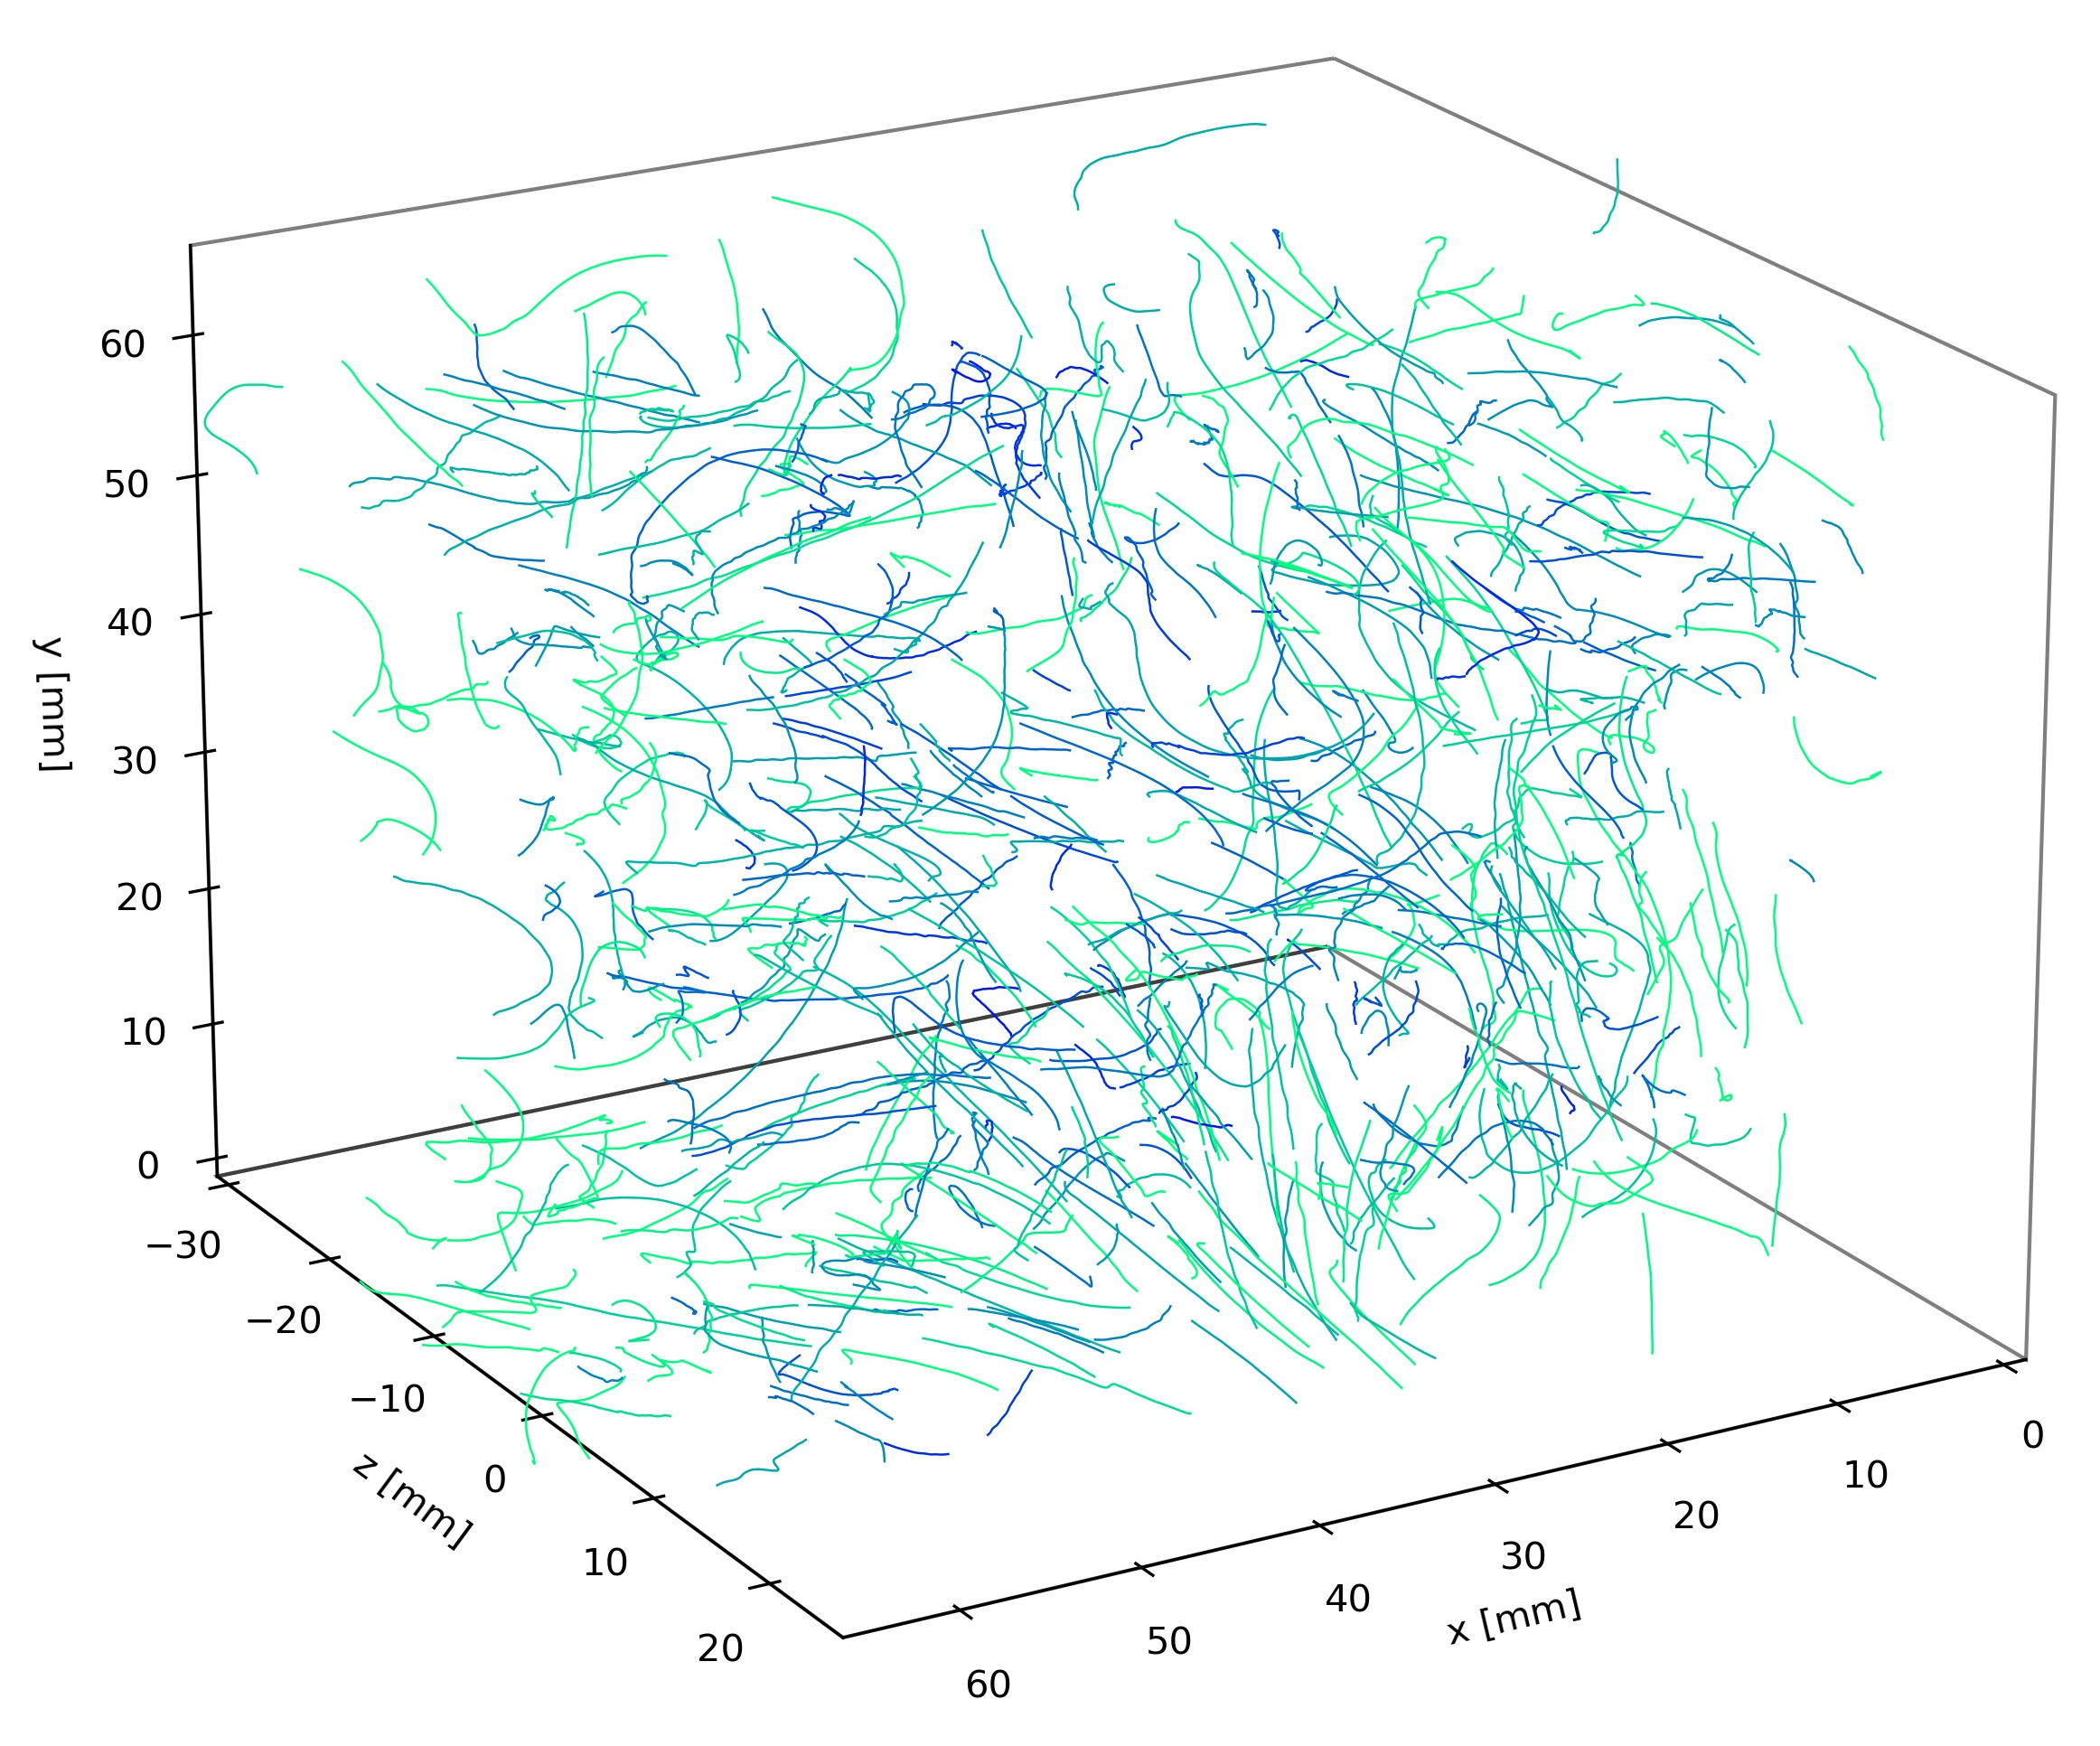
\includegraphics[width=10cm]{traj_image.jpg}
\end{center}

\vfill

\begin{minipage}{10cm}
	{\small 
	Vesrion: 0.2 \\
	Last updated: \today \\
	Github repository: \url{https://github.com/ronshnapp/MyPTV} \\
	Contac: ronshnapp@gmail.com}
\end{minipage}



\newpage
% ================================
%            TOC
% ================================
\tableofcontents
\pagenumbering{Roman}
\newpage

\pagenumbering{arabic}








% ================================
%            Section 1
% ================================


\section{Introduction}

\subsection{3D-PTV principles}


The 3D-PTV method is used to measure trajectories of particles in 3D space. It utilises the pronciples of stereoscopic vision in order to reconstruc 3D positions of particles from images taken from several angles. A scheme of a typical 3D-PTV experiment using a four camera system is shown in Fig.~\ref{fig:3dptv_exp}. The "work horse" behind the 3D-PTV method is the colinearity condition, the 3D model. In principle, if we know what is the position and what is the orientation of the camera in 3D space ($O'$ and $\theta$ in Fig.~\ref{fig:3dmodel}), we can use the pin-hole camera model to relate the image space coordinates of a particle ($\eta,\, \zeta$ in Fig.~\ref{fig:3dmodel}) to the ray of light connecting the imaging center and the particle. Then, if we have more than one camera, the particle will be located at the intersection of the two rays. Detailed information is given in \cite{Virant1997, Mass1993}.  


\begin{figure}[h!]
	\centering
	\subfloat[]{\label{fig:3dptv_exp}
		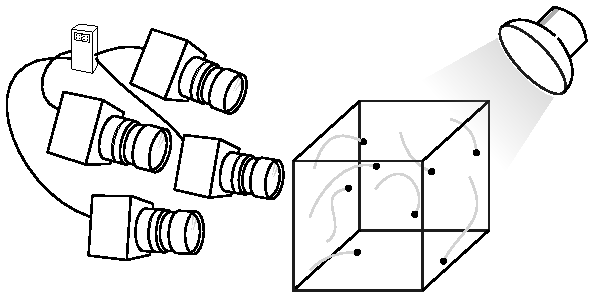
\includegraphics[width=6.5cm]{3D_PTV_acquisition.pdf}}
	\hfill
	%
	\subfloat[]{\label{fig:3dmodel}
		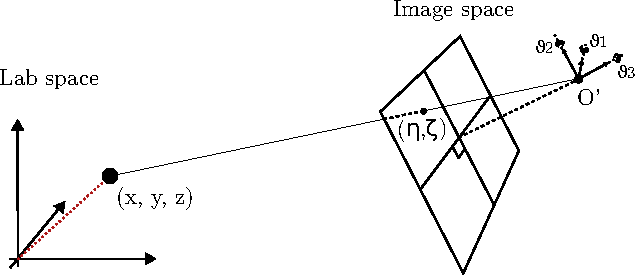
\includegraphics[width=6.5cm]{pinhole_model.pdf}}
	%
	\caption{(a) A schematics of a 3D-PTV experiment. (b) A schematic description of the 3d model, the pin-hole camera model.}
\end{figure}



Once the experiment, namely data aquisition, is done, there are six intrinsic steps to follow in order to complete the analysis. The six steps are outlined in Fig.~\ref{fig:steps}. In Camera calibration, we use images of known calibration targets to estimate the position, orientation and internal parameters of the cameras. In particle segmentation we use image analysis to obtain the paritlces' image space coordinates ($\eta, \, \zeta$). In the Particle matching step we use the ray crossing principle to decide which particle image in each of the cameras correspond to the same physical particle, and triagulate their positions through stereo mathcing. In particle tracking we connect the positions of particles in 3D space to form trajectories. In data conditioning we might use smoothing and re-tracking algorithms to enhance the quality of our data according to some physical heuristics. Lastly, we can analyze the data to obtain information on the physics of the particles we are studying. The MyPTV package is meant to handle the first five of these steps.    



\begin{figure}
	\centering
	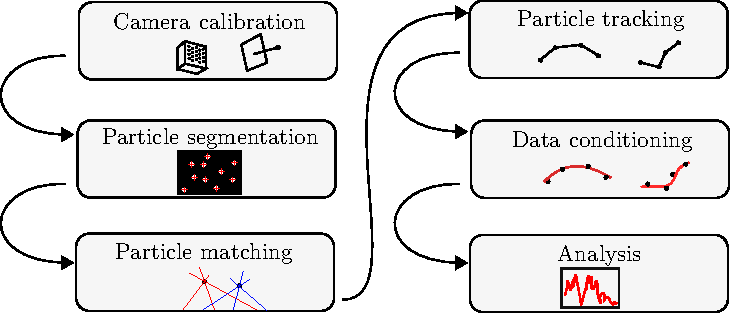
\includegraphics[width=10cm]{steps.pdf}
	\caption{Basic steps in the analysis of PTV raw data into particl trajectories and scientific output. The first five steps are handled by MyPYV. \label{fig:steps}}
\end{figure}


The sections that follow outline the code used to handle the 3D-PTV method in MyPTV.





\subsection{3D model}


To transform the 2D particles seen in camera images we use a pinhole camera model. In particular, the following expretion relates the coordinates in the 2D image space coordinates and a direction vector pointing out from the camera imaging center:
%
\begin{equation}
\vec{r}-\vec{O} = \Big( \, 
\begin{bmatrix}
\eta + x_h\\
\zeta + y_h \\
f
\end{bmatrix}
+ \vec{e}(\eta, \zeta) \,\Big) \cdot \Big[ R \Big]
\label{eq:3dmodel}
\end{equation}
%
where the description of the notations is given in Table~\ref{tab1:mathdesc}. The matrix $[R]= [R_1]\cdot [R_2] \cdot [R_3]$ is the rotation matrix calculated with the components of the orientation vector, $\vec{\theta} = [\theta 1,\, \theta 2,\, \theta 3]$. In addition, the correction temr $\vec{e}$ is assumed to be a quadratic polynomial of the image space coordinates:
%
\begin{equation}
\vec{e}(\eta,\,\zeta) = [E]\cdot P(\eta,\,\zeta) =
\begin{bmatrix}
E_{11} & E_{12} & E_{13} & E_{14} & E_{15}\\
E_{21} & E_{22} & E_{23} & E_{24} & E_{25}\\
0 & 0 & 0 & 0 & 0
\end{bmatrix}
\cdot 
\begin{bmatrix}
\eta\\
\zeta\\
\eta^2\\
\zeta^2\\
\eta\,\zeta
\end{bmatrix}
\end{equation}
%
where $[E]$ is a $3\times5$ matrix that holds the correction coefficients; the last row is filled with zeros because we do not attempt to correct $f$.





\begin{table}[h]
	\centering
	\caption{Description of mathematical notation. \label{tab1:mathdesc}}
	\begin{tabular}{p{5em} p{30em}}
		\hline
		Symbol & Description \\ \hline
		$\vec{r}$ & Particle position in the lab space coorindates\\
		$\vec{O} $& Position of a camera's imaging center \\
		$\eta, \, \zeta$ & image space coordinates (pixels) of a particle \\
		$x_h , \, y_h$ & Correction to the camera's imaging center (in pixels)\\
		$f$ & The camera's principle distance divided by the pixel size \\ 
		$\vec{e}(\eta, \zeta)$ & A nonlinear correction term to compensate for image distortion and multimedia problems.\\
		$[R]$ & The roation matrix which corresponds to the camera orientation vector. \\  \hline
	\end{tabular}
\end{table}















\subsection{MyPTV usage and structure}


MyPTV is used to conduct the post processing steps in which the experimental raw data - images - are transformed into particles' trajectories. The five steps include camera calibration, image segmentation, particle matching, particle tracking, and, data conditioning which is divided into smooting and stitching of broken trajectories. This section outlines how these steps are to be followed and how MyPTV is stuctured to fascilitate them. Section~\ref{sec:workflow} gives instructions on how to efficiently use MyPTV. 


At the current stage MyPTV does not include a graphical user interface. Instead, the package includes a script that can be used to efficienty and conveniently run the various steps in the post processing. Knowledge in Python is not required to operate MyPTV.



Each of the steps described above is dealt with in MyPTV as a separate "module". Each module consists of a Python script file which includes one or several classes. Detailed information on each of these classes is given in Sections~\ref{sec:image_mod}--\ref{sec:stitching}, and the code itself includes documentation to a level apropriate for development. In addition to the source code, MyPTV includes a \textit{workflow} script that is used to operate the software in an organized fasion. Thus, MyPTV can either be used either by using the workflow script, or by directly evoking classes from the source code. 







\clearpage



\section{The Workflow}\label{sec:worflow}


Operation of MyPTV can be fascilitated using the \texttt{workflow.py} script. The script is found under the \textit{example} folder under the home directory of the MyPTV package. The workflow is used through command line given instructions and a file that outlines the parameters to be used in each step.





\subsection{Preparation of an experiment folder}

To begin post processing of the 3D-PTV results, please follow these steps:

\begin{enumerate}
	\item Prepare a new directory; place inside of it the experiment data: the calibration images in a directory called \texttt{Calibration} and the particle images under separate folders named after the name of each camera.
	\item Locate the \texttt{example} under the root folder of the MyPTV package. This can be used as a template to the experiment directory made in the previous step.
	\item Copy the files \texttt{workfolw.py} and \texttt{params\char`_file.yml} from the \texttt{example} folder into your experiment's folder.
\end{enumerate}




\subsubsection{The \texttt{workflow.py} script}

\texttt{workflow.py} is a Python script used by the user to run the various steps of the experiment. It is used through the terminal or commend line. To use the various functions, use the following syntex:
\begin{verbatim}
cd \path\to\experiment\folder
python workflow.py params_file.yml "command"
\end{verbatim}
where \texttt{"command"} should be replaced with one of the following options, depending on the particular step of the post processing:
%
\begin{verbatim}
	calibration
	match_target_file
	segmentation
	matching
	tracking	
	smoothing
	stitching
\end{verbatim}



\subsubsection{The \texttt{params\char`_file.yml} file}

The \texttt{params\char`_file.yml} outlines all the parameters needed in order to run MyPTV using the workflow script. Thus, in every step conducted go through the lists of parameters and make sure that their values are correct. The definitions are tabulated per every step in the sections below.







\subsection{Calibration}

A good calibration is key to having success in your PTV experiment! Thus, follow this guide to calibrate your camera using myptv.


First, we need to prepare a \textit{target file}. This is a text file which lists the lab-space cooredinates of all the points on our calibration target according to the format shown in Fig.~\ref{fig:target_file}. Prepare such a file and save it in the experiment's calibration folder.


Then, each camera in MyPTV is calibrated separately. Thus, to calibrate a camera, we make sure that we have a calibration image ready (as seen in Fig.~\ref{fig:cal_img}, for example). Then, we perform an initial "rough" calibration, and finish of with the final calibration. 


\begin{figure}[h]
	\centering
	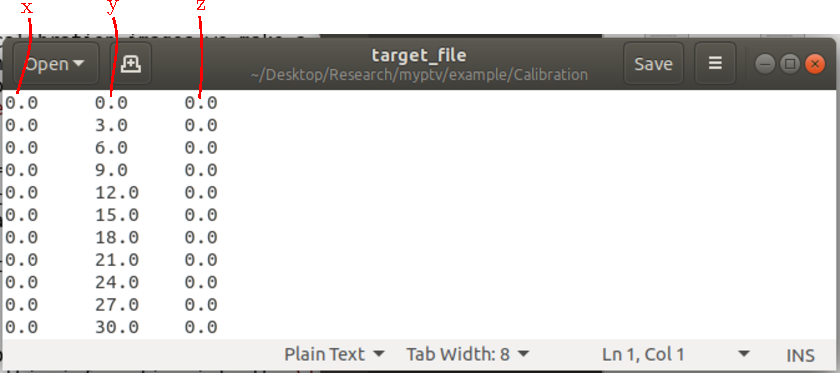
\includegraphics[width=10cm]{target_file.pdf}
	\caption{Format of the target file, which lists the lab-space coordinates of the calibration target as tab-separated values. The order at which points are given is not relevant. \label{fig:target_file}}
\end{figure}


\begin{table}
\centering
\caption{The \texttt{params\char`_file.yml} parameters for the calibration step. All paths to files are relative to the \texttt{workflow.py} script.}
\begin{tabular}{l m{10cm}}
	\hline
	Parameter & Description\\
	\hline
	\texttt{camera\char`_name} & the name of the camera to be calibrated \\
	
	\texttt{calibration\char`_points\char`_file} & path to the file that lists the correlated lab space and image space coordinates \\
	
	\texttt{target\char`_file} & path to the file that lists the calibration target's lab points \\
	
	\texttt{segmented\char`_points\char`_file} & path of the file with segmented calibration points \\
	
	\texttt{calibration\char`_image} & path of the calibration image \\
	
	\texttt{resolution} & camera resolution; for example: 1280, 1024\\
	\hline
\end{tabular}
\end{table}




\subsubsection{Initial calibraiton}

For each of the calibration images we make a \textit{calibration points file}. This is a file which lists the coorediantes of the calibration target points in both lab sapce and image space coordinates. These text files follow a simple tab-separated format as shown in Fig.~\ref{fig:calpointfile}. Therefore:
%
\begin{enumerate}
	\item Make a new text file. Name it, for example \texttt{cal\char`_points\char`_cam1}. Alternatively, copy the file from the \texttt{example/calibration} folder in MyPTV.
	
	\item Open the calibration image using an image viewer/editor (e.g. Microsoft paint, GIMP, Photoshop, or with matplotlib through \texttt{plt.imshow(plt.imread('path/to/image'))}).
	
	\item Choose about 6 points on the calibration target; measure their image space coordinates using the image editor and insert this information into the \textit{calibration points file}. Save and close the file.
	
	\item Once the \textit{calibration points file} is ready, calibrate the camera through the calibration scheme as outlined in Sec.~\ref{sec:cam_cal}.
\end{enumerate}
%

The initial "rough" calibration is now finished. 


\begin{figure}
	\centering
	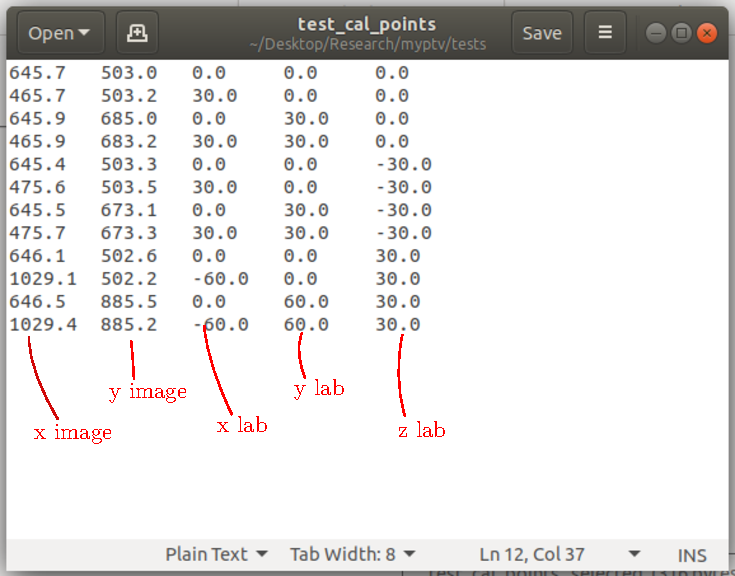
\includegraphics[width=10cm]{cal_point_file.pdf}
	\caption{An example of a text file holding the calibration point data. \label{fig:calpointfile}}
\end{figure}






\subsubsection{Segmenting the calibration images and matching the target file}


To prepare for the final calibration, we need to prepare a \textit{calibration points file} for the rest of the calibration points on our target. To avoid inserting the information for each point manualy, we use a semi-automated process as follows:
%
\begin{enumerate}
	\item Segment the calibration target points in the calibration image using the workflow script, as outlined in Sec.~\ref{sec:workflow_segment}. Save the segmented calibration points in the experiment's Calibration folder with a name such as \texttt{blobs\char`_cam1}. Insert the name of this file under the \texttt{segmented\char`_points\char`_file} field of the \texttt{params\char`_file.yml} file.
	
	\item Open the command line on the experiment directory, and run the workflow script with the following command:
	\begin{verbatim}
	python workflow.py params_file.yml match_target_file
	\end{verbatim}
	
	\item After automated sorting, a figure window should appear. Make sure that the blue points are overlaid with the red X's and close the figure window. Follow the instructions to save the calibration points file (under the name given in the \texttt{params\char`_file.yml} under\\ \texttt{calibration\char`_points\char`_file}). 
\end{enumerate}

You should now have a file that contains the full information of the calibration points. Proceed with the fine calibration process.






\subsubsection{Calibration workflow}\label{sec:cam_cal}


Once all the data files are ready in the exeriment folder, we use the workflow script to minimize the calibration error by tuning the cameras' external parameters and correction terms. Thus:

\begin{enumerate}
	
	\item Start a terminal (or command line prompt), and change directory to the experiment's folder:
	\begin{verbatim}
	cd \path\to\the\experiment\folder
	\end{verbatim}
	
	\item Enter the following command:
	\begin{verbatim}
	python workflow.py params_file.yml calibration
	\end{verbatim}
	
	\item If a camera file does not yet exist in the folder, MyPTV had just generated an empty one for you. Locate this file in the experiment folder, enter an initial guess for the external parameters and save the file.
	
	\item If a camera file exists in the exprimental folder, an interactive dialogue should now appear in the terminal which offers:
	\begin{verbatim}
	1 - external parameters minimization 
	2 - correction error term calibration
	3 - print current camera parameters
	4 - plot the projection of the calibration points
	8 - save the current calibration results
	9 - quit
	\end{verbatim}
	Thus, proceed using options 1 and 2 in iterations and note the calibration error decreasing. Once satisfied, save the results.
	
\end{enumerate}
	
* Note, a "good" calibration will have a low error value - less than 0.5 pixels. 

** Optional validation - After all the cameras have been calibrated, it is also good practice to verify the calibration solution by stereo matching the calibration points. To do this, we use the \texttt{match\char`_blob\char`_files} (Section~\ref{sec:matching}) to stereo match the files of the segmented calibration target points. We can then calculate the so-called \textit{static calibration error} by computing the RMS of the distance between the triangulated calibration points and the real data from the target file. See Fig.~\ref{fig:cal_err} for an example. This validation step is not yet implemented in the workflow script.


\begin{figure}
	\centering
	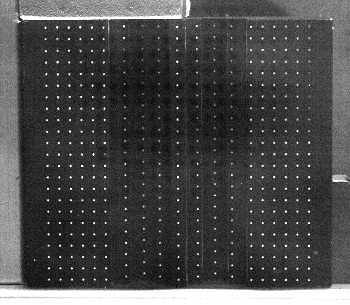
\includegraphics[width=5cm]{cal_image.jpg}
	\caption{An example of a calibration image. The points on the target have known lab space coordinates. Not also that the points are distributed over several plains (3 different $z$ values in this case). \label{fig:cal_img}}
\end{figure}


\begin{figure}
	\centering
	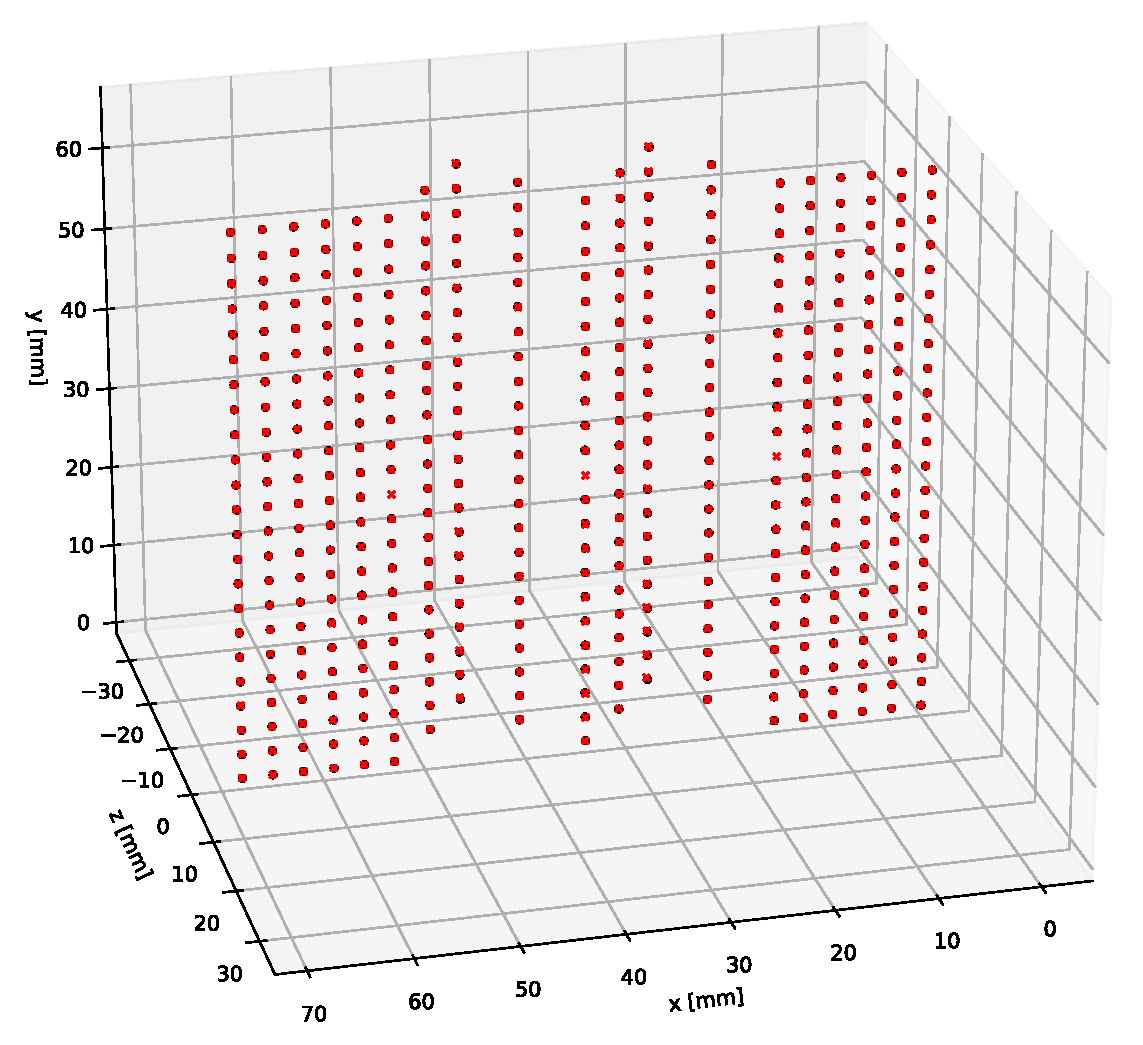
\includegraphics[width=6cm]{cal_error.pdf}
	\caption{An example plot of a calibration error estimation. The red crosses represent the known positions of the calibration points given in the target file, and the black circles mark the positions of the stereo-matched segmented calibration points. In this case, the root mean square of the static calibration error was 84$\mu m$. \label{fig:cal_err}}
\end{figure}






\subsection{segmentation}\label{sec:workflow_segment}


In this step we extract the particle coordinates in the images and save the coordinates in dedicated files. Use the \texttt{workflow.py} script with the \texttt{segmentation} command to start the process. 

\begin{enumerate}
	\item The segmentation is run first on a single image by specifying \texttt{Number\char`_of\char`_images: 1}. To view the results, use \texttt{plot\char`_result: True}, and make sure the results are not saved by using \texttt{save\char`_name: None}.
	
	\item Once the parameters are set for the first image, set \texttt{Number\char`_of\char`_images: None} to loop over all the images in the folder, and save the results by setting \texttt{save\char`_name: /file/name/to/use}
\end{enumerate}


\begin{table}[h]
	\centering
	\caption{The \texttt{params\char`_file.yml} parameters for the segmentation step. All paths to files are relative to the \texttt{workflow.py} script.}
	\begin{tabular}{l m{10cm}}
		\hline
		Parameter & Description\\
		\hline
		
		\texttt{Number\char`_of\char`_images} & Number of images over which to do the segmentation \\
		\texttt{images\char`_folder} & path to the folder containing the images\\
		
		\texttt{image\char`_extension} & extension of the images; for example, .tif\\
		
		\texttt{mask} & if this is 1.0, no mask is used; if this is set to a path to a file, the file will be used as a mask for the segmentation \\
		
		\texttt{ROI} & region of interest; specify by indicating the xmin, xmax, ymin, ymax coordinates \\
		
		\texttt{plot\char`_result} & if \texttt{False} will not plot the results; if \texttt{True} the results will be plotted \\
		
		\texttt{threshold} & the brightness value for which a point is considered a particle after a local threshold is performed \\
		
		\texttt{blur\char`_sigma} & the standard deviation of a Gaussian blur filter \\
		 
		\texttt{local\char`_filter} & the size of a local mean subtraction filter \\
		
		\texttt{min\char`_xsize} & minimum particle size (pixels) in $x$ direction \\
		
		\texttt{min\char`_ysize} & minimum particle size (pixels) in $y$ direction \\
		
		\texttt{min\char`_area} & minimum particle area (pixels$^2$)\\
		
		\texttt{max\char`_xsize} & maximum particle size (pixels) in $x$ direction \\
		
		\texttt{max\char`_ysize} & maximum particle size (pixels) in $y$ direction \\
		
		\texttt{max\char`_area} & maximum particle area (pixels$^2$) \\
		
		\texttt{save\char`_name} & if \texttt{None} the results will not be saved in a file; if \texttt{path/to/file} will save the results in the given file name \\
		
		\hline
	\end{tabular}
\end{table}






\subsection{matching}\label{sec:workflow_match}

In the matching step, particles images in the various images are used to stereo-locate (triangulate) the 3D positions of particles in the lab-space coordinates. As before, run first only on several images to find optimal parameter values, and only then interate over all frames by setting \texttt{N\char`_frames: None} and save the results. 


\begin{table}[h!]
	\centering
	\caption{The \texttt{params\char`_file.yml} parameters for the matching step. All paths to files are relative to the \texttt{workflow.py} script.}
	\begin{tabular}{l m{10cm}}
		\hline
		Parameter & Description\\
		\hline
		
		\texttt{blob\char`_files} & names of files that hold the segmented particles for each camera, separated by commas; for example: \texttt{blobs\char`_cam1, blobs\char`_cam2, blobs\char`_cam3} \\
		
		\texttt{N\char`_frames} & if \texttt{None} will match particles in all available frames; if an integer will match only particles in the first \texttt{N} frames. \\
		
		\texttt{camera\char`_names} & names of cameras used separated by commas; for example, \texttt{cam1, cam2, cam3} \\
		
		\texttt{cam\char`_resolution} & camera resolution; for example, \texttt{1280, 1024} \\
		
		\texttt{ROI} & region of interest for the matching in lab space coordinates, and according to the format of \texttt{xmin, xmax, ymin, ymax, zmin, zmax} \\
		
		\texttt{voxel\char`_size} & the side length of voxels used in the \textit{Ray Traversal} algorithm; note - too high values lead to long computation times and too low value result in matching errors and long computation times. \\
		
		\texttt{max\char`_blob\char`_distance} &  the distance particle usually undergo during each frame in image space coordinates (pixels)\\
		
		\texttt{max\char`_err} & maximum value of the RMS triangulation error in lab space coordinates \\
		
		\texttt{save\char`_name} & path name used for saving the results; if \texttt{None} the results are not saved \\
		
		\hline
	\end{tabular}
\end{table}





\subsection{tracking}\label{sec:workflow_track}

The tracking step is used to link particle in the lab space coordinates in time, thus forming the 3D trajectories.




\begin{table}[h!]
	\centering
	\caption{The \texttt{params\char`_file.yml} parameters for the tracking step. All paths to files are relative to the \texttt{workflow.py} script.}
	\begin{tabular}{l m{10cm}}
		\hline
		Parameter & Description\\
		\hline
		
		\texttt{particles\char`_file\char`_name} & path name of the file which holds the 3D coordinates of particles, namely the results of the matching step  \\
		
		\texttt{N\char`_frames} & if \texttt{None} will iterate over particles in all frames; if an integer will only track particles in the first \texttt{N} frames of the particles file\\
		
		\texttt{d\char`_max} & the maximum translation in lab space coordinates \\
		
		\texttt{dv\char`_max} & the maximum allowable change in velocity in lab scape coordinates per frame (e.g. mm/frame) \\
		
		\texttt{save\char`_name} & name of the file in which the results shall be saved; if \texttt{None} the reuslts are not saved on the hard drvie \\
		
		\hline
	\end{tabular}
\end{table}






\subsection{smoothing}\label{sec:workflow_smooth}


The smoothing step is used to smooth trajectories in time and to caluculate the velocity and acceleration of particles. This is done by fitting polynomials over sliding windows of the trajectory where velocities and acceleration are calculated through a direct differentiation of the polynomial (see~\cite{Luthi2005}).



\begin{table}[h!]
	\centering
	\caption{The \texttt{params\char`_file.yml} parameters for the smoothing step. All paths to files are relative to the \texttt{workflow.py} script.}
	\begin{tabular}{l m{10cm}}
		\hline
		Parameter & Description\\
		\hline
		
		\texttt{trajectory\char`_file} & file name of the trajectories file, namely the results of the tracking step \\
		
		\texttt{window\char`_size} & window size of the sliding polynomial \\
		
		\texttt{polynom\char`_order} & degree of the polynomial used in the smoothing \\
		
		\texttt{save\char`_name} & file name to save the results; if \texttt{None} the results will not be save on the disk \\
		
		\hline
	\end{tabular}
\end{table}

    
    


\subsection{stitching}\label{sec:workflow_stitch}

This step is used to re-track trajectories once velocities are known and to "stitch" broken trajectories following the algorithm of Ref.~\cite{Xu2008}.


\begin{table}[h!]
	\centering
	\caption{The \texttt{params\char`_file.yml} parameters for the smoothing step. All paths to files are relative to the \texttt{workflow.py} script.}
	\begin{tabular}{l m{10cm}}
		\hline
		Parameter & Description\\
		\hline
		
		\texttt{trajectory\char`_file} & name of the smoothed trajectory file used in the stitching \\
		
		\texttt{max\char`_time\char`_separation} & maximum time separation over which to stitch broken trajectories \\
		
		\texttt{max\char`_distance} & maximum distance in the position-velocity space \\
		
		\texttt{save\char`_name} & file name to save the results; if \texttt{None} the results will not be save on the disk \\
		
		\hline
	\end{tabular}
\end{table}












\clearpage


\section{Imaging module - \texttt{imaging\char`_mod.py}}\label{sec:image_mod}


The imaging module is used to handle the translation from 2D image space coordinates to lab spcae coordinates and vice-versa through the 3D model. 



\subsection{The \texttt{camera} object}\label{sec:camera}

An object that stores the camera external and internal parameters and handles the projections to and from image space and lab space. Inputs are:

\begin{enumerate}
	\item \texttt{name} - string, name for the camera. This is the name used when saveing and loading the camera parameters.
	\item \texttt{resolution} - tuple (2), two integers for the camera number of pixels
	\item \texttt{cal\char`_points\char`_fname} - string (optional), path to a file with calibration coordinates for the camera. The format fro the calibration point file is given in Section~\ref{sec:calpointreader} (see Fig.~\ref{fig:calpointfile}).
\end{enumerate}


The important functionalities are:


\begin{enumerate}
	\item \texttt{get\char`_r(eta, zeta)} - Will solve eq.~\ref{eq:3dmodel} for the orientation vector $\vec{b} = \vec{r} - \vec{O}$, given an input of pixel coordinates $(\eta, \, \zeta)$.
	
	\item \texttt{projection(x)} - Will reverse solve equation~\eqref{eq:3dmodel} to find the image space coordinates $(\eta, \, \zeta)$, of an input 3D point, (\texttt{x=}$\vec{r}$).
	
	\item \texttt{save(dir\char`_path)} - Will save the camera parameters in a file called after the camera name in the given directory path, see Fig.~\ref{fig:camfiles}.
	
	\item \texttt{load(dir\char`_path)} - Will load the camera parameters in a file called after the camera name in the given directory path, see Fig.~\ref{fig:camfiles}.
\end{enumerate}



After calibration we can save the camera parameters on the hard disc. The camera files have the structure shown in Fig.~\ref{fig:camfiles}.

\begin{figure}[h]
	\centering
	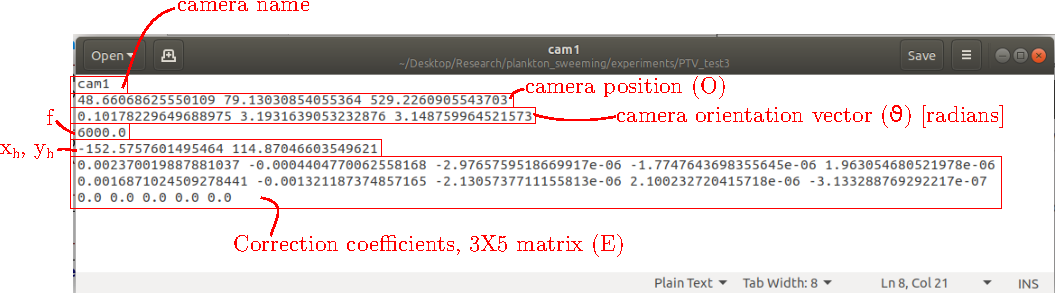
\includegraphics[width=\textwidth]{camera_files.pdf}
	\caption{The structure of a camera file. The files are simple text files where each row corresponds to a specific paramter and the values in each row are separated by a whitespace. \label{fig:camfiles}}
\end{figure}








\subsection{The \texttt{imsys} object}


An object that holds several camera instances and can be used to perform stereo-matching. The important functionalities are:


\begin{enumerate}
	\item \texttt{stereo\char`_match(coords, d\char`_max)} - Takes as an input a dicionary with coordinates in image space from the several cameras and calculates the triagulation position. \\ The coordinate dicitonary has keys that are the camera number and the values which are the coordinates in each camera. d\char`_max is maximum allowable distance for the triangulation.
	
\end{enumerate}








\subsection{The \texttt{Cal\char`_image\char`_coord} object}\label{sec:calpointreader}

This is a class used for reading information given in the optional argument \texttt{cal\char`_points\char`_fname} of the \texttt{camera} class (Sec.~\ref{sec:camera}). It is used internally and generally users will not have to deal with this. This class will read and interpret text files with tab separated valued, where the columns' meanings are: [x image space, y image space, x lab space, y lab space, z lab space], and each row is a single point of some known calibration target.

The input for this class is:
\begin{enumerate}
	\item \texttt{fname} - String, the path to your calibration point file. The file is holds tab separated values with the meaning of: [x image, y image, x lab, y lab, z lab], see Fig.~\ref{fig:calpointfile}.
\end{enumerate}








\section{Camera calibration - \texttt{calibrate\char`_mod.py}}


The \texttt{calibrate\char`_mod.py} module, with the \texttt{calibrate} object, is used to find the camera calibration parameters. We calibrate each camera by taking an image of a \textit{calibration target} - a body with markings of known coordinates in lab space - and search for the camera parameters that minimize the distance between the projection of the known points in image space and the image taken with the camera. 



\subsection{The \texttt{calibrate} object}

Used to solve for the camera parameters given an input list of image space and lab space coordinates. The inputs are:

\begin{enumerate}
	\item \texttt{camera} - An instance of a \texttt{camera} object which we would like to calibrate.
	\item \texttt{lab\char`_coords} - a list of lab space coordinates of some known calibration target. 
	\item \texttt{img\char`_coords} - a list of image space coordinates that is ordered in accordance with the lab space coordinates. 
\end{enumerate}



The important functionalities are:
%
\begin{enumerate}
	
	\item \texttt{searchCalibration(maxiter=5000, fix\char`_f=True)} - When this is run, we use a nonlinear least squares search to find the camera parameters that minimize the cost function (item 3 below). This function is used to find the $\vec{O}$, $\vec{\theta}$, $f$, and $x_h, \, y_h$ parameters (in case \texttt{fix\char`_f=False}, it will not solve for $f$. \texttt{maxiter} is the maximum number of iterations allowed for the least squares search.
	
	\item \texttt{fineCalibration(maxiter=500)} - This function will solve for the coefficients of the quadratic polynomial used for the nonlinear correction term ($[E]$). 
	
	\item \texttt{mean\char`_squared\char`_err} - This is our cost function, being the sum of distances between the image space coordinates and the projection of the given lab space coordinates.
	
\end{enumerate}
%
To find an optomal calibration solution, we might need to run each function several times, and run the coarse and fine calibrations one after the other until a satisfactory solution is obtained. Once it is obtained, we should keep in mind to save the results using the \texttt{save} functionality of the \texttt{camera} object. 











\section{Particle segmentation - \texttt{segmentation\char`_mod.py}} 


This module handles the image analysis part of MyPTV, taking in raw camera images containing particles and outputing their image space coordinates. For the segmentation we first blur the image to remove salt and pepper noise, then we highlight particles using a local mean subtraction around each pixel, and then use a global threshold to mark foreground and backgroud pixels. Finally, the connected foreground pixels are considered to be particles, and we estimate the blob's center using a brightness weighted average of blob pixels.



\subsection{The \texttt{particle\char`_segmentation} object} 

Used to segment particles in a given image. This class is used internally to iterate over frames in a single folder by the \texttt{loop\char`_segmentation} class. However, it is usefull to check the segmentation parameters manually using this \texttt{particle\char`_segmentation} over several images in order to tune the particle searching. The inputs are:
%
\begin{enumerate}
	\item \texttt{image} - the image for segmentation
	\item \texttt{sigma=1.0} - the standard deviation of the blurring filter
	\item \texttt{threshold=10} - the global filter's threshold brightness value (pixels with brightness higher than this number are considered foreground) 
	\item \texttt{mask=1.0} - A mask matrix can be used to specify rigions of interest within the image
	\item \texttt{local\char`_filter=15} - The window size (pixels) for the local filter.
	\item a bunch of threshold pixel sizes in all directions and in area.
\end{enumerate}


The important funcitonalities are:
%
\begin{enumerate}
	\item \texttt{get\char`_blobs} - Will return a list of blob centers, their box size and their area.
	
	\item \texttt{plot\char`_blobs()} - Uses matplotlib to plot the results of the segmentation. A very usefull functionality in the testing of segmentation parameters!
	
	\item \texttt{save\char`_results(fname)} - Will save the segmented particles in a text file. The file is arranged in six columns with the following attributes: (x center position, y center position, x size, y size, area, image number), see Fig.~\ref{fig:blobfile}.
\end{enumerate}






\subsection{The \texttt{loop\char`_segmentation} object} 


An object used for looping over images in a given directory to segment particles
and save the results in a file.


important functionalities are:
%
\begin{enumerate}
	\item \texttt{segment\char`_folder\char`_images()} - Will loop over the images in the given directory and segment particles according to the given parameters
	\item \texttt{save\char`_results(fname)} - Will save the segmented particles in a text file. The file is arranged in six columns with the following attributes: (x center position, y center position, x size, y size, area, image number), see Fig.~\ref{fig:blobfile}.
\end{enumerate}

\begin{figure}[h!]
	\centering
	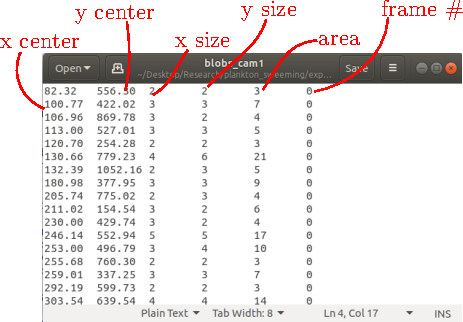
\includegraphics[width=10cm]{blob_file.pdf}
	\caption{An example of a text file holding the segmentation resuls and the description of the different columns. \label{fig:blobfile}} 
\end{figure}








\section{Particle matching - \texttt{particle\char`_matching\char`_mod.py}} \label{sec:matching}

The module used to link particles in the different images through stereo matching and estimating their 3D positions. One of the main issue in this process is that stereo matching all possible candidates is an NP hard problem, so to track numerous particles in each frame we have to choose which particles are likely to produce a 3D particle coordinate. Thus, particle matching in MyPTV uses two algorithms in conjunction. First is a novel algorithm that uses 2D time tracking of blobs to deduce which candidates are more likely to produce trackable particles in 3D. Second is the Ray Traversal algorith proposed in Ref~\cite{Bourgoin2020}, in which the lab space volume is devided to voxels and stereo matching is attempted for rays within each voxel. Using the two algorithms in conjunction was found to yield a 50\% reduction in conputational time and more trackable trajectories (45\% more trajectories were found in a test). 




\subsection{The \texttt{match\char`_blob\char`_files} object}


This is the object that we use to get trangulated particles results from the segmented blob files (a file as the one in Fig.~\ref{fig:blobfile} for each camera). For each frame it first runs the first algorithm using time information, and only then uses the Ray traversal algorithm on the blobs that were not successfully connected. The inputs are:
%
\begin{enumerate}
	\item \texttt{blob\char`_fnames} - a list of the (srting) file names containing the segmented blob data. The list has to be sorted according the order of cameras in the \texttt{img\char`_system}.
	
	\item \texttt{img\char`_system} - an instance of the \texttt{img\char`_system} class with the calibrated cameras.
	
	\item \texttt{RIO} - A nested list of 3X2 elements. The first holds the minimum and  maximum values of $x$ coordinates, the second is same for $y$, and  the third for $z$ coordinates. 
	
	\item \texttt{voxel\char`_size} - the side length of voxel cubes used in the ray traversal algorithm. Given in lab space coordinates (e.g. mm). Note - a too large voxel size will result in high computational times due a high number of candidates, while a too small voxel size might lead to erronous intersection of rays, leading to matching errors. Thus, this parameter should be optimized.
	
	\item \texttt{max\char`_blob\char`_dist} - the largest distance for which blobs are concidered neighbours in the image space coordinates (namely, the largest permissible blob displacement in pixels).
	
	\item \texttt{max\char`_err=None} - Maximum acceptable uncertainty in particle position. If None, (defult), than no bound is used.
	
	\item \texttt{reverse\char`_eta\char`_zeta=False} - Should be false if the eta and zeta coordinates need to be in reverse order so as to match the calibration. This may be needed if the calibration data points were given where the x and y coordinates are transposed (as happens, e.g., if using matplotlib.pyplot.imshow).
\end{enumerate}


The important functionalities are:
%
\begin{enumerate}
	\item \texttt{get\char`_particles()} - Use this to match blobs into particlesin 3D.
	\item \texttt{save\char`_results(fname)} - Save the results in a text file. The format has 4 + number of cameras columns separated by tabs:
	(x, y, z, [N columns corresponding to the blob number in each camera] , frame number, see Fig.~\ref{fig:particlefile}).
\end{enumerate}



\begin{figure}[h!]
	\centering
	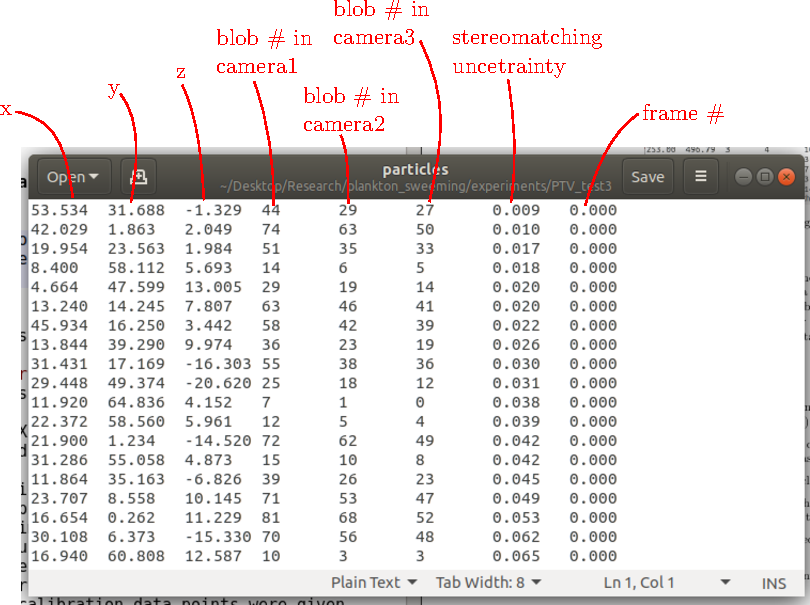
\includegraphics[width=12cm]{particle_file.pdf}
	\caption{An example of a text file holding the triangulated particles' resuls and the description of the different columns. In this example there were three cameras. \label{fig:particlefile}} 
\end{figure}




\subsection{The \texttt{matching} object}

This object is the "engine" used to match particles using the Ray Traversal algorithm. In practice we run the relevant functions: \texttt{get\char`_voxel\char`_dictionary()} $\rightarrow$ \texttt{list\char`_candidates()} $\rightarrow$ \texttt{get\char`_particles()}, and after that the results are held in the attribute \texttt{matched\char`_particles}.




\subsection{The \texttt{matching\char`_using\char`_time} object}

This object performs the matching of blobs using the 2D tracking heuristic. In principle, it is given a list of blobs that were successfully used to form 3D particles in the previous frame. Then, for each of the given blobs it searches for nearest neighbours in the current frame, and stereo-matches those blobs that were found (using the \texttt{.triangulate\char`_candidates()} method). 





\subsection{The \texttt{initiate\char`_time\char`_matching} object}

This object is used to initiate the time searching algorithm on the first frame. It goes over the blobs at the first frame and searches for blobs that have nearest neighbours at the second frame. Those that have neighbours are used in a first run of the Ray Traversal algorithm, thus they are given priority in the search.













\section{Tracking in 3D - \texttt{tracking\char`_mod.py}}

This is the module that is used to track particles in 3D. There are currently three tracking methods implemented, nearest neighbour, two-frame, and four-frame, see Ref.~\cite{Ouellette2006}. Users are welcome to choose their perfered method and use it.



\subsection{The \texttt{tracker\char`_four\char`_frames} object}\label{sec:four_frames}

An object used to perform tracking through the 4-frame best estimate method \cite{Ouellette2006}. Input:
%
\begin{enumerate}
	\item \texttt{fname} - a string name of a particle file (e.g. Fig.~\ref{fig:particlefile}
	\item \texttt{mean\char`_flow=0.0} - either zero (deafult) of a numpy array of the mean flow vector, in units of the calibrations spatial units per frame (e.g. mm per frame). The mean flow is assumed not to change in space and time.
	\item \texttt{d\char`_max\char`=1e10} - maximum allowable translation between two frames for the nearest neighbour search, after subtracting the mean flow. 
	\item \texttt{dv\char`_max\char`=1e10} - maximum allowable change in velocity for the two-frame velocity projection search. The radius around the projection is therefore dv\char`_max/dt (where dt = 1 frame$^{-1}$)
\end{enumerate}


The important functionalities are:
%
\begin{enumerate}
	\item \texttt{track\char`_all\char`_frames()} - Will track particles through all the frames. 
	
	\item \texttt{return\char`_connected\char`_particles()} - Will retun the list of trajectories that were established.
	
	\item \texttt{save\char`_results(fname)} - Will save the results on the hard drive. The results are saved in a text file, where each row is a sample of a trajectory. The columns are specified as follows: [trajectory number, x, y, z, frame number], see Fig~\ref{fig:trajfile}.  
\end{enumerate}

\begin{figure}
	\centering
	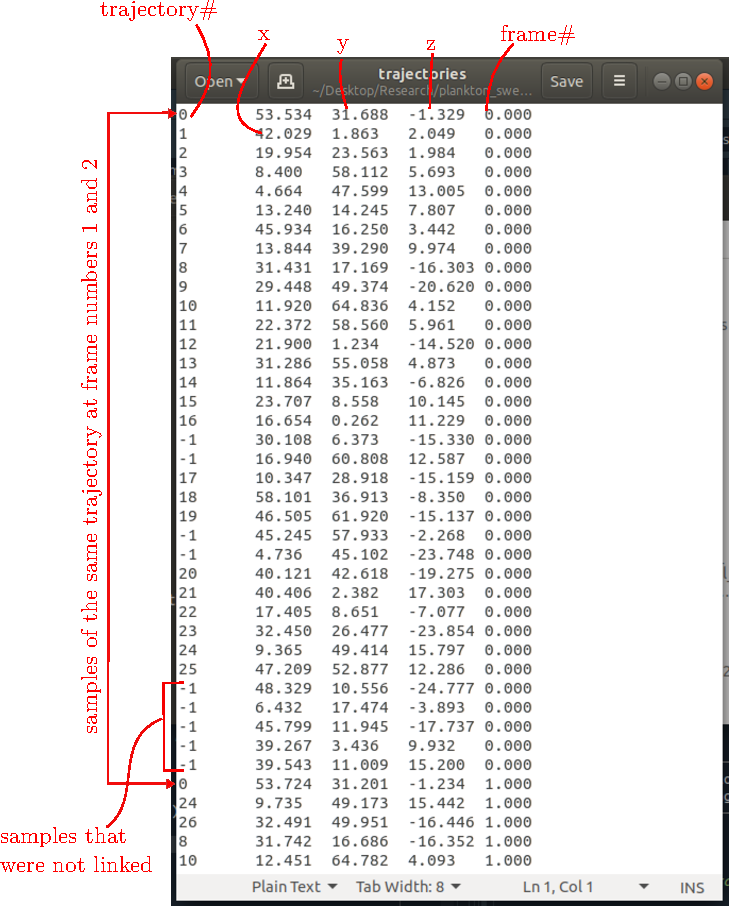
\includegraphics[width=10cm]{trajectory_files.pdf}
	\caption{Example of a trajectory file and the column definitions. \label{fig:trajfile}}
\end{figure}




\subsection{The \texttt{tracker\char`_two\char`_frames} object}

An object used for tracking through the 2-frame method. The description is the same as in Section~\ref{sec:four_frames}



\subsection{The \texttt{tracker\char`_nearest\char`_neighbour} object}

An object used for tracking through the nearest neighbour method. The description is the same as in Section~\ref{sec:four_frames}









\section{Trajectory smoothing - \texttt{traj\char`_smoothing\char`_mod.py}}

This module is used to smooth trajecotries and to calculate the velocity and acceleration of the particles. For the smoothing we are using the polynomial fitting methd proposed and used in Refs.~\cite{Luthi2005, Shnapp2019}. In short, each component of the particle's position is fitted with a series of polynomials with a sliding window of fixed lenght and the derivatives are calculated by analytically differentiating the polynomial. The end result is a new file with smoothed trajectories. However note that we smooth and calculate valocities and accelerations only for trajectories longer than the window size for the smoothing (a user decided parameter). 


\subsection{The \texttt{smooth\char`_trajectories} object}

A class used to smooth trajectories in a list of trajectories. Due to the smoothing we also calculate the velocity and acceleration of the trajectories. The input trajecotry list structure is the same as the files produced by the classes in \texttt{tracking\char`_mod.py}.

Note - only trajectories whose length is larger than the window size will be smoothed and saved. Shorter trajectories are svaed with zero velocity and accelerations.


The inputs are:
\begin{enumerate}
	\item \texttt{traj\char`_list} -  a list of samples organized as trajecotries. This should have the same data structure used in the saving function of the tracking algorithms (see Section~\ref{sec:four_frames}). 
	\item \texttt{window} - The window size used in the sliding polynomial fitting.
	\item \texttt{polyorder} - The order of the polynomial used in the fitting. 
\end{enumerate}

\begin{figure}[h!]
	\centering
	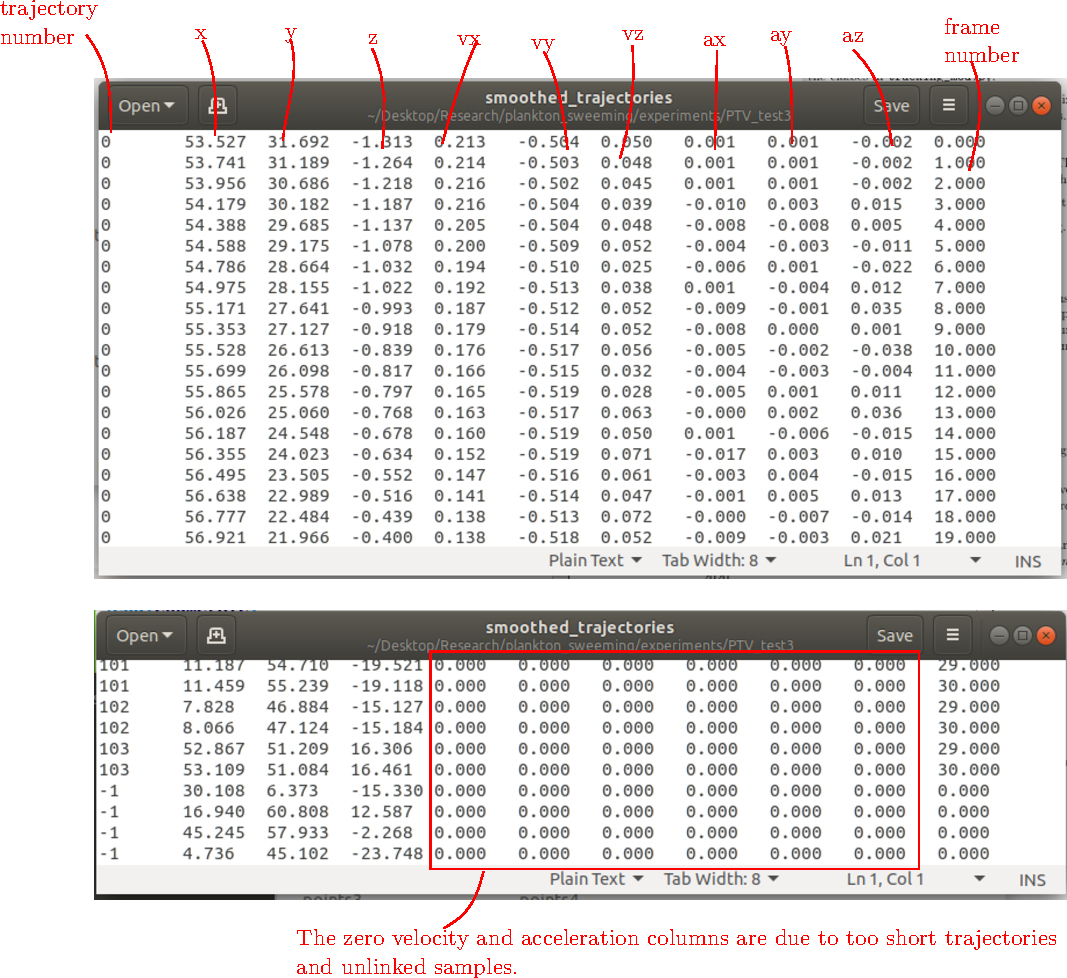
\includegraphics[width=12cm]{smoothed_trajfile.pdf}
	\caption{Example file holding the results of smoothed trajectories, and the description for each column. Note also the unsmoothed samples at the bottom of the file. \label{fig:smoothedfile}}
\end{figure}

The important functionalities are:

\begin{enumerate}
	\item \texttt{smooth()} - performs the actual smoothing
	\item \texttt{save\char`_results(fname)} - Saves the results on the hard drive using the given (string) file name. The resulting file is a text file such that each row is a sample of a trajectory, and with 11 columns. The columns have the following meaning:
	[traj number, $x$, $y$, $z$, $v_x$, $v_y$, $v_z$, $a_x$, $a_y$, $a_z$, frame number], where $v_i$ and $a_i$ denote components of the velocity and acceleration vectors respectively, see Fig.~\ref{fig:smoothedfile}.
\end{enumerate}







\section{Trajectory stitching - \texttt{traj\char`_stitching\char`_mod.py}}\label{sec:stitching}

This module applies the algorithm by REf.~\cite{Xu2008} to connect trajectories that were broken along the process by tracking the trajectories again in the position--velocity space. We also extend this by interpolating the missing samples using a 3rd order polynomial, that is fitted to the existing 4 data points at the tips of the broken trajectories. This module is applied after the trajectory smoothing step.




\subsection{The \texttt{traj\char`_stitching} object}

This object performs the stitching process. Inputs:

\begin{enumerate}
	\item \texttt{traj\char`_list} - the list of smoothed trajectory, given as a Numpy array of shape (N,11), where N is the number of samples. The format is the same as the format generated after the smoothing process.
	\item \texttt{Ts} - The maximum number of broken samples allowed in the connection.
	\item \texttt{dm} - The maximum distance between the trajectory for which connections are made.
\end{enumerate}



The important functionalities are:

\begin{enumerate}
	\item \texttt{stitch\char`_trajectories()} - Will search for candidates and stitch the best fitting candidates. Run this function to perform the stitching. After running the new trajectory list is held as the attribute \texttt{new\char`_traj\char`_list}.
	
	\item \texttt{save\char`_results(fname)} - Will save the stitched trajectories in a text file with a given file name. The format for the saved file is the same as the one used in the smoothing trajectories (Fig.~\ref{fig:smoothedfile}).
\end{enumerate}





\bibliography{bib_myPTV}
\bibliographystyle{unsrt}

\end{document}